% Generated, editable TikZ figures for the diagram specifications kept in
% comment environments in IT_report.tex.
\definecolor{reportblue}{RGB}{42,92,145}
\definecolor{reportgreen}{RGB}{58,125,101}
\definecolor{reportorange}{RGB}{207,128,45}
\definecolor{reportred}{RGB}{176,69,64}

\tikzset{
  reportbox/.style={draw=#1!85!black, fill=#1!12, rounded corners=3pt,
    minimum height=1.15cm, text width=2.25cm, align=center, font=\scriptsize},
  reportarrow/.style={-{Latex[length=2.2mm]}, thick, draw=black!65},
  block/.style={draw=reportblue!85!black, fill=reportblue!12, rounded corners=3pt,
    thick, minimum width=2.5cm, minimum height=1.25cm, align=center, font=\small},
  subblock/.style={draw=reportblue!85!black, fill=reportblue!12, rounded corners=2pt,
    thick, minimum width=1cm, minimum height=1cm, align=center, font=\small},
  arrow/.style={-{Latex[length=2.2mm]}, thick, draw=black!65}
}

\newcommand{\ReportFlow}[8]{%
  \begin{figure}[H]
    \centering
    \begin{tikzpicture}[node distance=4mm]
      \node (a) [reportbox=#2] {#3};
      \node (b) [reportbox=#2, right=of a] {#4};
      \node (c) [reportbox=#2, right=of b] {#5};
      \node (d) [reportbox=#2, right=of c] {#6};
      \node (e) [reportbox=#2, right=of d] {#7};
      \draw[reportarrow] (a) -- (b);
      \draw[reportarrow] (b) -- (c);
      \draw[reportarrow] (c) -- (d);
      \draw[reportarrow] (d) -- (e);
    \end{tikzpicture}
    \caption{#1}\label{#8}
  \end{figure}%
}

\newcommand{\ReportStack}[8]{%
  \begin{figure}[H]
    \centering
    \begin{tikzpicture}[node distance=4mm]
      \node (a) [reportbox=#2, text width=.62\textwidth] {#3};
      \node (b) [reportbox=#2, text width=.62\textwidth, below=of a] {#4};
      \node (c) [reportbox=#2, text width=.62\textwidth, below=of b] {#5};
      \node (d) [reportbox=#2, text width=.62\textwidth, below=of c] {#6};
      \node (e) [reportbox=#2, text width=.62\textwidth, below=of d] {#7};
      \draw[reportarrow] (a) -- (b);
      \draw[reportarrow] (b) -- (c);
      \draw[reportarrow] (c) -- (d);
      \draw[reportarrow] (d) -- (e);
    \end{tikzpicture}
    \caption{#1}\label{#8}
  \end{figure}%
}

\newcommand{\ReportBars}[3]{%
  \begin{figure}[H]
    \centering
    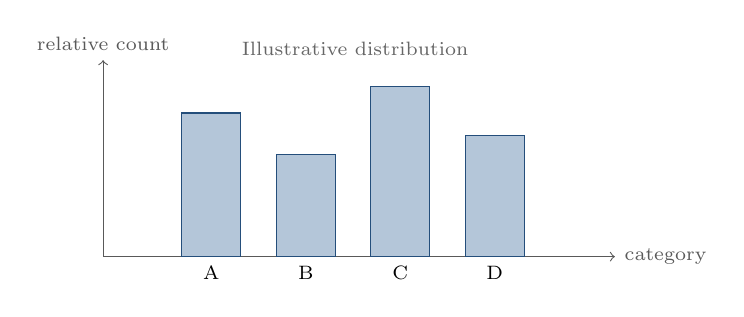
\begin{tikzpicture}[x=1cm,y=.48cm, font=\scriptsize]
      \draw[->,black!65] (0,0) -- (6.5,0) node[right] {category};
      \draw[->,black!65] (0,0) -- (0,5.2) node[above] {relative count};
      \foreach \x/\h/\t in {1/3.8/A,2.2/2.7/B,3.4/4.5/C,4.6/3.2/D}{
        \filldraw[fill=reportblue!35,draw=reportblue!85!black] (\x,0) rectangle +(0.75,\h);
        \node[below] at (\x+.375,0) {\t};
      }
      \node[align=center, text=black!60] at (3.2,5.5) {Illustrative distribution};
    \end{tikzpicture}
    \caption{#1}\label{#3}
  \end{figure}%
}

\newcounter{reportdiagram}
\newcommand{\ReportCommentFigure}{%
  \stepcounter{reportdiagram}%
  \ifcase\value{reportdiagram}\or
    \ReportFlow{Evolution of communication networks from conventional architectures to intelligent AI-driven 5G ecosystems.}{reportblue}{Conventional networks}{Cellular networks}{Software-defined networking}{Cloud-native 5G}{AI-driven ecosystems}{fig:network_evolution}%
  \or \ReportFlow{Overall internship workflow and engineering pipeline.}{reportblue}{Requirements study}{Mininet simulation}{RSNSD engineering}{SliceNet design}{Evaluation and roadmap}{fig:overall_workflow}%
  \or \ReportStack{Methodology adopted during the internship.}{reportblue}{Knowledge acquisition}{Simulation and hybrid data acquisition}{RSNSD dataset engineering}{SliceNet model development}{Experimental evaluation}{fig:methodology}%
  \or \ReportFlow{Evolution of mobile communication technologies from analog cellular systems to intelligent AI-enabled 5G networks.}{reportblue}{1G\\Analog voice}{2G\\Digital voice}{3G\\Mobile data}{4G\\Mobile broadband}{5G\\AI-enabled services}{fig:mobile_generations}%
  \or \ReportFlow{High-level architecture of a modern 5G communication network.}{reportblue}{User equipment}{Radio access network}{5G core\\control and user plane}{Edge and cloud services}{AI management and orchestration}{fig:5g_architecture}%
  \or \ReportFlow{Major functional entities within the 5G Core Network.}{reportblue}{User equipment}{gNodeB}{AMF / SMF\\control plane}{UPF\\user plane}{Data networks}{fig:5g_core}%
  \or \ReportFlow{Representative rural communication network deployment.}{reportgreen}{Rural users and IoT}{Local access network}{Private 5G RAN}{Local edge and 5G core}{Public and cloud services}{fig:rural_network}%
  \or \ReportFlow{Traditional 5G network slicing architecture over a shared physical infrastructure.}{reportorange}{Service requests}{eMBB slice}{URLLC slice}{mMTC slice}{Shared physical infrastructure}{fig:traditional_slicing}%
  \or \ReportFlow{Application-oriented service-aware network slicing framework.}{reportgreen}{Service traffic}{Service classification}{QoS and context mapping}{Logical service slices}{Shared 5G infrastructure}{fig:service_slicing}%
  \or \ReportFlow{AI-assisted network management workflow.}{reportblue}{Traffic monitoring}{Feature extraction}{AI inference}{Resource allocation}{Slice configuration}{fig:ai_networking}%
  \or \ReportFlow{Machine learning pipeline for traffic classification.}{reportblue}{Traffic flows}{Feature vectors}{Training data}{Classifier}{Service prediction}{fig:ml_pipeline}%
  \or \ReportFlow{Closed-loop self-healing network architecture.}{reportgreen}{Network telemetry}{Anomaly detection}{Diagnosis}{Recovery action}{Performance feedback}{fig:self_healing}%
  \or \ReportFlow{Limitations of conventional network management approaches.}{reportred}{Static policies}{Generic slice classes}{Limited rural data}{Manual optimisation}{Poor adaptability}{fig:current_limitations}%
  \or \ReportFlow{Motivation behind the proposed service-aware networking framework.}{reportorange}{5G applications}{Rural challenges}{Research gaps}{Simulation and RSNSD}{AI service model}{fig:research_motivation}%
  \or \ReportFlow{Engineering roadmap of the proposed project.}{reportblue}{Requirements study}{Simulation platform}{RSNSD engineering}{SliceNet perception}{Future autonomy}{fig:engineering_roadmap}%
  \or \ReportFlow{Overall project architecture for intelligent service-aware networking.}{reportblue}{Rural services}{Mininet simulation}{RSNSD dataset}{SliceNet classifier}{Intelligent orchestration}{fig:overall_architecture}%
  \or \ReportFlow{Experimental environment architecture.}{reportblue}{Service hosts}{Mininet topology}{Open vSwitch}{Traffic monitor}{Dataset storage}{fig:experimental_environment}%
  \or \ReportFlow{Mininet simulation architecture used during the internship.}{reportblue}{Traffic generators}{Mininet hosts}{Open vSwitch}{Controller}{Flow monitoring}{fig:simulation_architecture}%
  \or \ReportFlow{Rural Mininet topology.}{reportgreen}{Rural service hosts}{Access switch}{Aggregation switch}{Gateway}{External services}{fig:mininet_topology}%
  \or \ReportStack{Service-aware traffic generation pipeline.}{reportgreen}{Healthcare, education, agriculture and general-service profiles}{Traffic profile generator}{Packet generation}{Mininet transmission and monitoring}{Captured traffic for RSNSD}{fig:traffic_generation}%
  \or \ReportFlow{Feature extraction pipeline used for generating RSNSD.}{reportblue}{Captured packets}{Packet parsing}{Flow aggregation}{Feature computation}{RSNSD records}{fig:feature_pipeline}%
  \or \ReportFlow{Complete dataset generation workflow adopted during the internship.}{reportblue}{Mininet traffic}{Synthetic traffic}{Schema harmonisation}{Feature and label engineering}{RSNSD v1.0}{fig:dataset_pipeline}%
  \or \ReportFlow{Motivation for the Rural Service-aware Network Slice Dataset (RSNSD).}{reportorange}{Rural diversity}{QoS heterogeneity}{Dataset gap}{Hybrid data engineering}{RSNSD v1.0}{fig:dataset_motivation}%
  \or \ReportFlow{RSNSD generation pipeline.}{reportgreen}{Scenario definitions}{Simulation acquisition}{Synthetic generation}{Schema harmonisation}{Labeled RSNSD}{fig:rsnsd_pipeline}%
  \or \ReportFlow{Simulation-based data acquisition workflow.}{reportblue}{Scenario configuration}{Mininet execution}{Service traffic}{Flow capture}{Simulation samples}{fig:simulation_pipeline}%
  \or \ReportFlow{Synthetic data generation workflow.}{reportorange}{Statistical profiles}{Parameter sampling}{Synthetic flows}{Quality checks}{Synthetic samples}{fig:synthetic_pipeline}%
  \or \ReportFlow{Schema harmonisation pipeline for RSNSD.}{reportgreen}{Simulation schema}{Synthetic schema}{Field standardisation}{Validation}{Unified RSNSD schema}{fig:schema}%
  \or \ReportFlow{Scenario distribution represented in RSNSD.}{reportblue}{Normal operation}{High demand}{Congestion}{Emergency response}{Disaster recovery}{fig:scenario_distribution}%
  \or \ReportFlow{RSNSD feature engineering pipeline.}{reportblue}{Raw traffic}{Packet parsing}{Flow aggregation}{Feature validation}{Final feature vector}{fig:rsnsd_feature_engineering}%
  \or \ReportStack{Automatic label generation workflow for RSNSD.}{reportgreen}{Simulation configuration}{Service and scenario mapping}{QoS priority mapping}{Network slice mapping}{Labeled RSNSD record}{fig:label_generation}%
  \or \ReportStack{Dataset validation and quality-assurance workflow.}{reportblue}{Schema validation}{Completeness checks}{Range and consistency checks}{Class-balance assessment}{Validated RSNSD}{fig:validation}%
  \or \ReportBars{Simulation vs synthetic sample contribution.}{reportblue}{fig:source_distribution}%
  \or \ReportBars{Packet size distribution.}{reportblue}{fig:packet_distribution}%
  \or \ReportBars{Flow duration distribution.}{reportblue}{fig:flow_distribution}%
  \or \ReportBars{Bandwidth utilization across service categories.}{reportblue}{fig:bandwidth}%
  \or \ReportFlow{Position of SliceNet within the intelligent networking framework.}{reportblue}{Mininet simulation}{RSNSD v1.0}{SliceNet\\perception layer}{Context and slice selection}{Future RL and self-healing}{fig:slicenet_framework}%
  \or \ReportFlow{Service classification problem formulation adopted for SliceNet.}{reportblue}{Network flow}{Engineered feature vector}{Feature preprocessing}{SliceNet}{Service-class prediction}{fig:classification_problem}%
  \or \ReportStack{Feature preprocessing pipeline used before training SliceNet.}{reportblue}{Raw RSNSD features}{Missing-value and type checks}{Encoding categorical attributes}{Normalisation}{Model-ready feature vectors}{fig:feature_preprocessing}%
  \or \ReportFlow{Architecture of the proposed SliceNet neural network.}{reportblue}{Input features}{Dense layer + ReLU}{Batch norm + dropout}{Dense layer + ReLU}{Softmax service classes}{fig:slicenet_architecture}%
  \or \ReportStack{Training workflow adopted for SliceNet.}{reportblue}{RSNSD dataset}{Train, validation and test split}{Model optimisation}{Validation and tuning}{Final test evaluation}{fig:training_workflow}%
  \or \ReportFlow{Future evolution of the proposed intelligent networking framework beyond the internship.}{reportgreen}{SliceNet predictions}{Context engine}{Slice selection}{RL resource allocation}{Autonomous self-healing}{fig:future_pipeline}%
  \fi
}

% Emit an editable figure immediately before each existing commented specification,
% then preserve the specification itself as non-typeset source documentation.
\let\ReportOriginalComment\comment
% \begin{comment} opens a local group before it invokes \comment.  Schedule
% the figure after the original implementation closes that group; otherwise a
% float created here is discarded along with the commented material.
\renewcommand{\comment}{\aftergroup\ReportCommentFigure\ReportOriginalComment}
